\chapter{評価}
\label{chap:evaluation}

本章では、本研究で実装したインスリンデバイスと食事検知デバイスのそれぞれの性能を評価する。
そしてその二つの評価結果について論じた後、二つを合わせてインスリン打ち忘れ通知に関する評価とその結果をもとに考察を述べる。

\section{インスリンデバイス}
インスリンデバイスの性能について評価をし、考察する。

\subsection{評価環境}
インスリンペンデバイスを評価するための実験環境について述べる。

\subsection{誤検知率}
誤検知率がどれくらいになったのかを述べる。

\begin{figure}[htbp]
  \caption{インスリン注射器に装着したデバイスの誤検知率}
  \label{fig:success_failure_rate_insulin}
  \begin{center}
    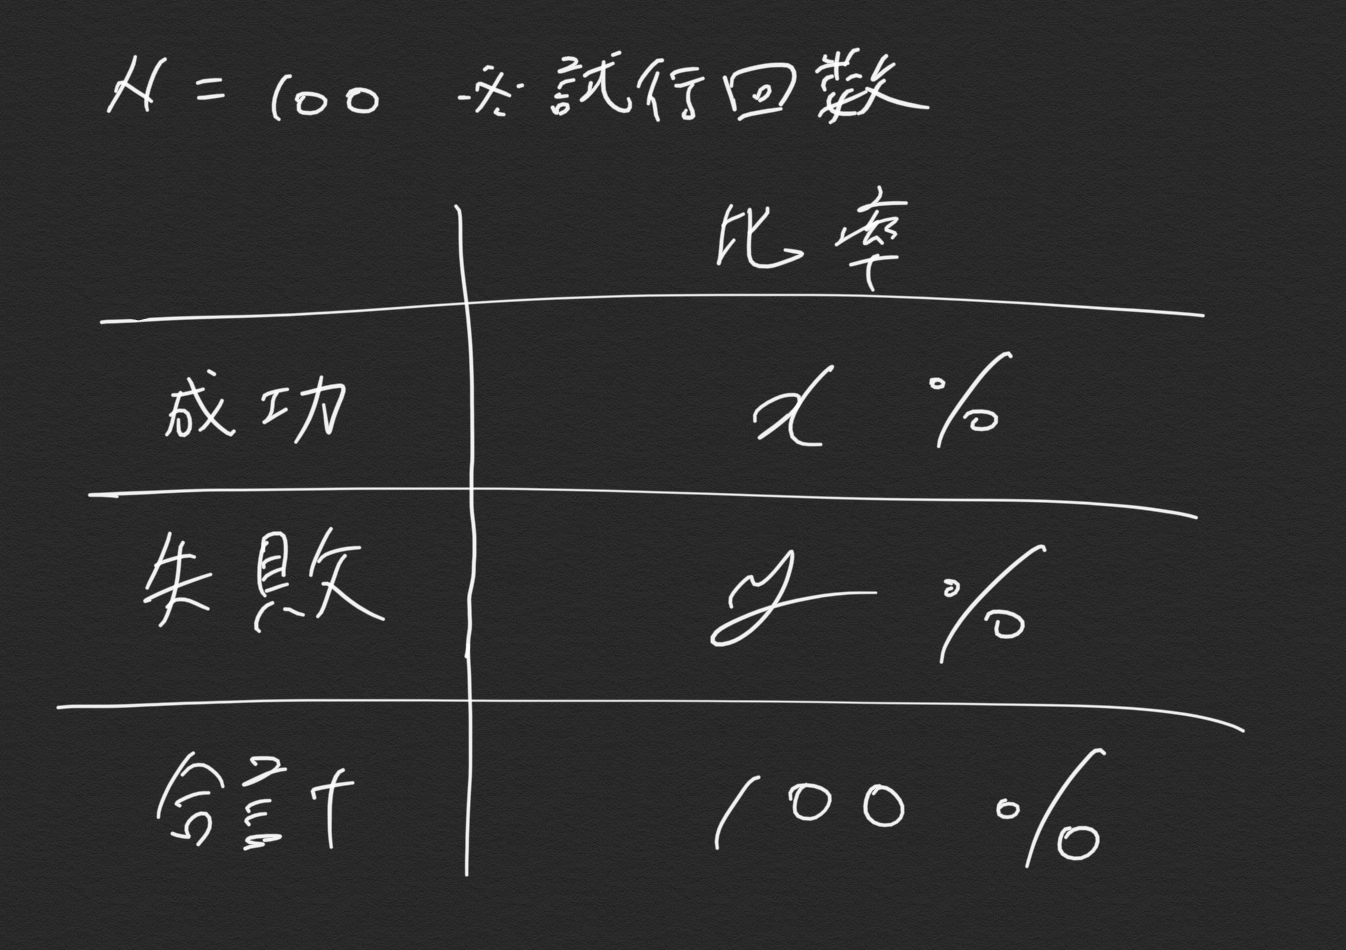
\includegraphics[bb=0 0 1000 450,width=20cm]{assets/success_failure_rate.png}
  \end{center}
\end{figure}

\subsection{検知時間と実摂取時間の差異}
検知時間と実際に摂取した時間にどれくらい誤差があるのかを見る。

\begin{figure}[htbp]
  \caption{インスリン注射器に装着したデバイスによる検知の時間誤差}
  \label{fig:insulin_box_n_whisker}
  \begin{center}
    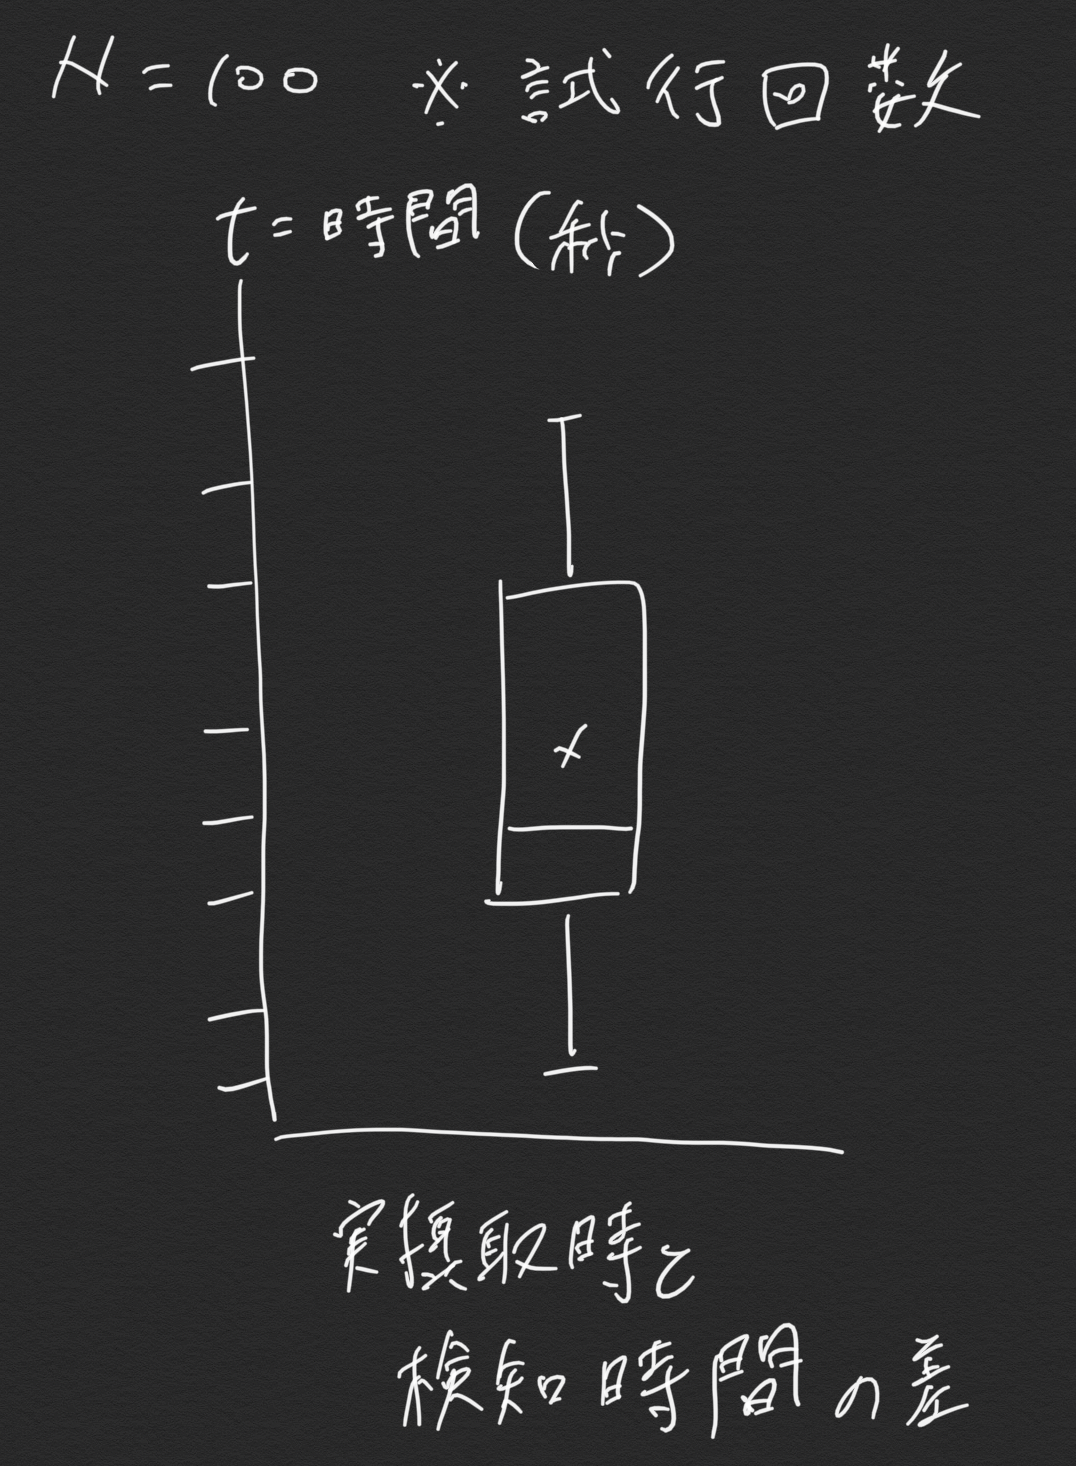
\includegraphics[bb=0 0 1000 850,width=20cm]{assets/insulin_box_n_whisker.png}
  \end{center}
\end{figure}

\section{食事検知}
食事検知の性能について評価をし、考察する。

今回対象とする、卓上での行動は以下の通りである。

\begin{enumerate}
  \item 食事
  \item 読書
  \item スマホを触る
  \item パソコンで作業する
  \item ゲームする
  \item ものを書く
  \item お茶を飲む
  \item 机を拭く
  \item 机そのものを移動する
\end{enumerate}

\subsection{評価環境}
食事検知を評価するための実験環境について述べる。

\subsection{誤検知率}
誤検知率がどれくらいになったのかを述べる。

\begin{figure}[htbp]
  \caption{加速度による食事検知の誤検知率}
  \label{fig:success_failure_rate_meal}
  \begin{center}
    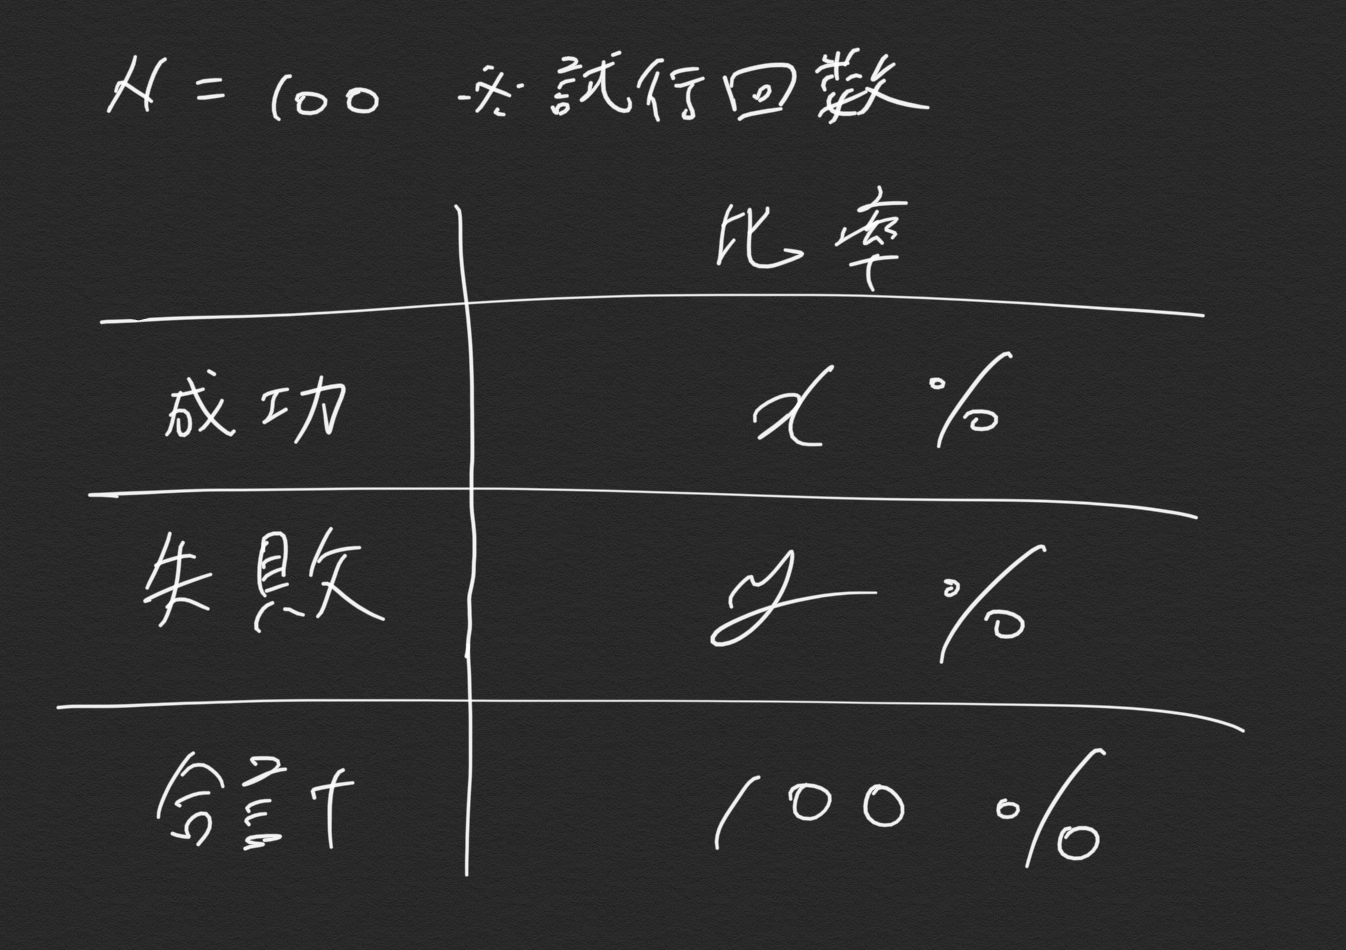
\includegraphics[bb=0 0 1000 450,width=20cm]{assets/success_failure_rate.png}
  \end{center}
\end{figure}

\subsection{検知時間と実摂取時間の差異}
検知時間と実際に食事をとった時間にどれくらい誤差があるのかを見る。

\begin{figure}[htbp]
  \caption{加速度による食事検知の時間誤差}
  \label{fig:meal_box_n_whisker}
  \begin{center}
    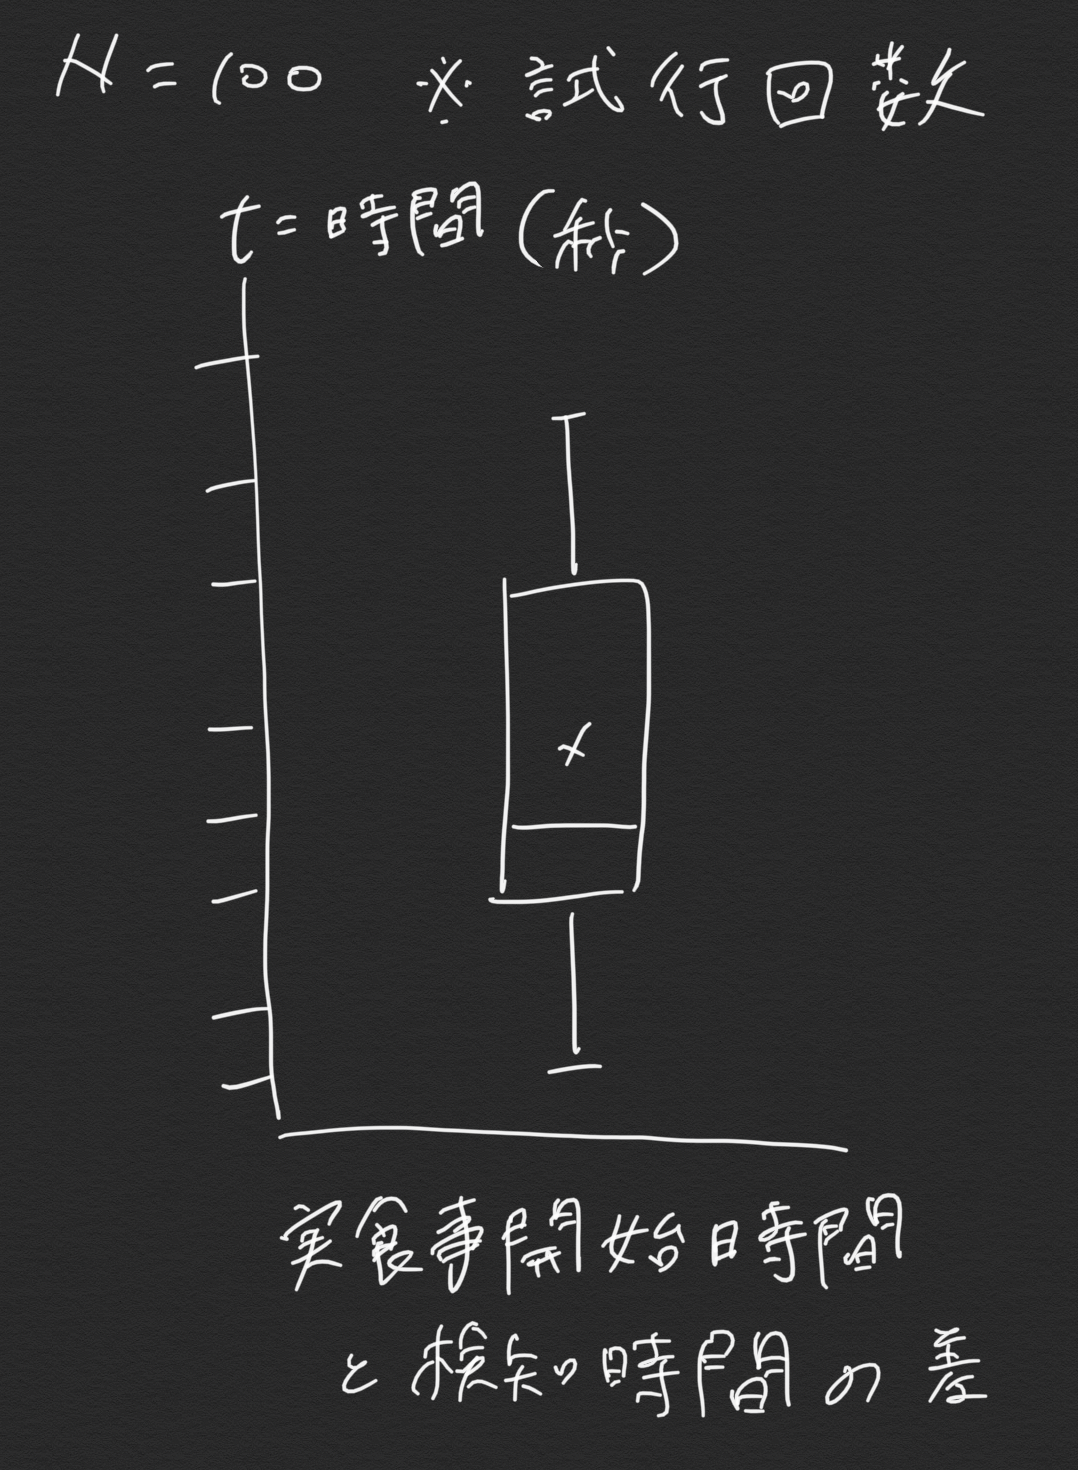
\includegraphics[bb=0 0 1000 850,width=20cm]{assets/meal_box_n_whisker.png}
  \end{center}
\end{figure}

\section{インスリン摂取忘れ通知}
上記2つの評価をもとに、インスリン摂取忘れ通知が達成できるかどうかについて評価し、考察する。

\subsection{評価環境}
インスリン摂取忘れ通知の評価をするための実験環境について述べる。

被験者は手元に記録用媒体を準備し、シナリオ別にアラート音声を聞いたかどうか、またどのタイミングで聞いたかを記録する。

\subsection{シナリオ}

本研究では、以下の二つを実験シナリオとして実施した。

\begin{enumerate}
  \item 被験者は、第\ref{chap:implementation}章、第\ref{section:insulin_pen_device}節にて実装されたデバイスが装着されたインスリン注射器を使用して、食前にインスリン投与と同じアクションを行う。投与のアクションを終えたのち、食事を開始する。
  \begin{description}
    \item[期待する結果]\mbox{}\\
      インスリン注射器に装着されたデバイスが送信した投与時間は食事検知時間よりも前で、インスリンが正常に投与されたものとして判定。アラートの音声は発されない。
  \end{description}
  \item 被験者は、第\ref{chap:implementation}章、第\ref{section:insulin_pen_device}節にて実装されたデバイスが装着されたインスリン注射器を使用することなく、食事を始める。
  \begin{description}
    \item[期待する結果]\mbox{}\\
      食事検知時に直近30分で、インスリンが正常に投与されなかったものとして判定。アラートの音声が発される。
  \end{description}
\end{enumerate}

\begin{figure}[htbp]
  \caption{シナリオ実験結果(回数)}
  \label{fig:notify_success_failure}
  \begin{center}
    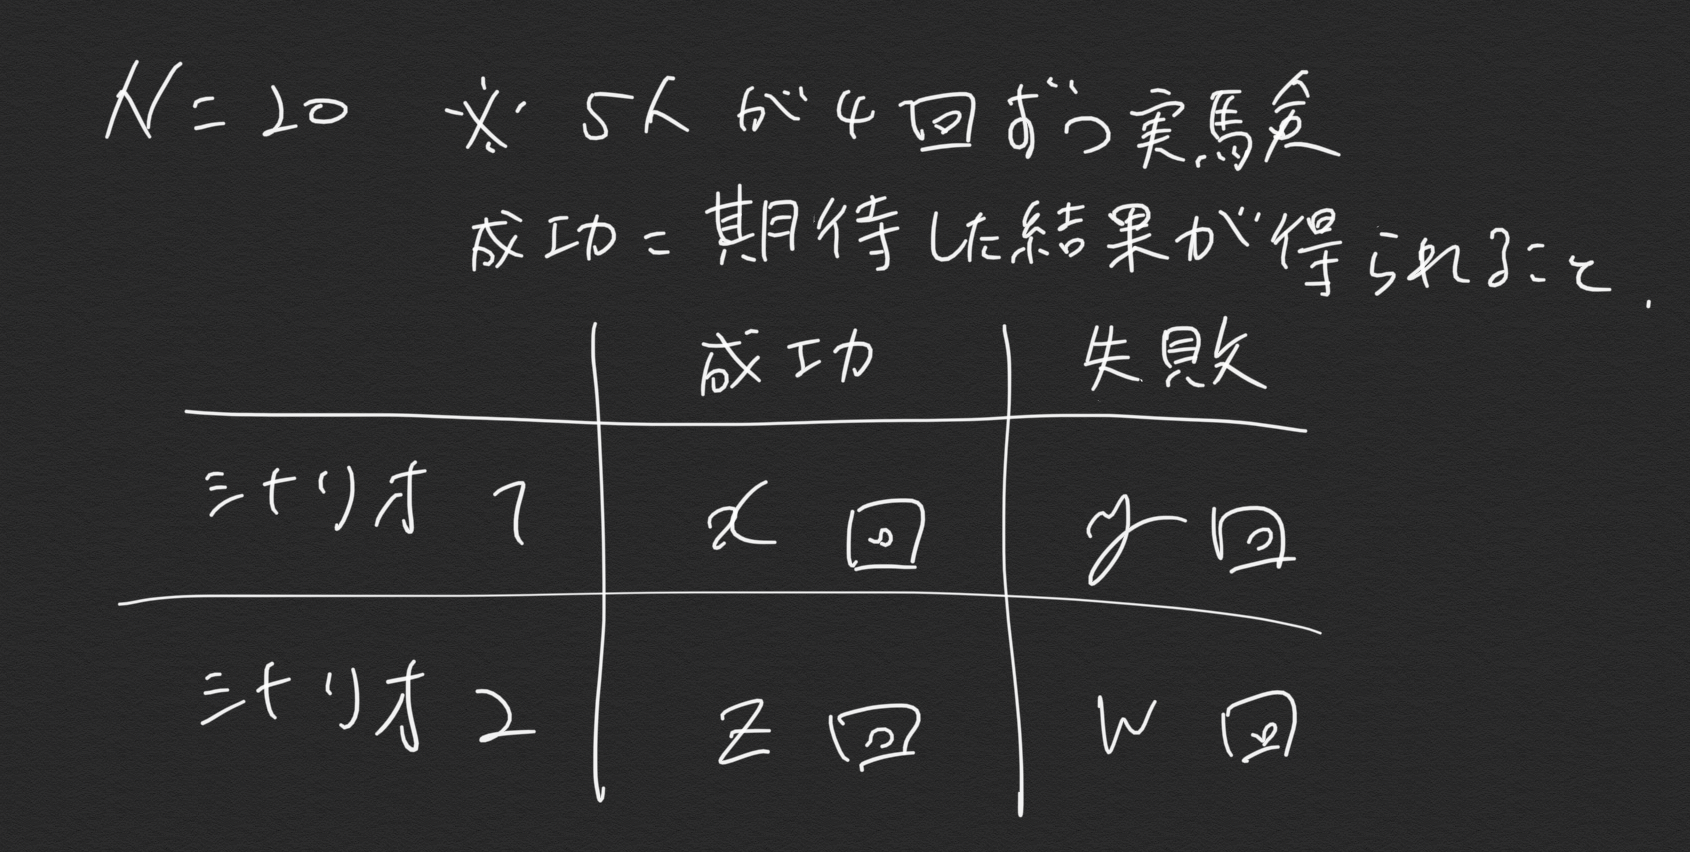
\includegraphics[bb=0 0 1000 400,width=20cm]{assets/notify_success_failure.png}
  \end{center}
\end{figure}

\begin{figure}[htbp]
  \caption{シナリオ実験結果(百分率)}
  \label{fig:notify_success_failure_rate}
  \begin{center}
    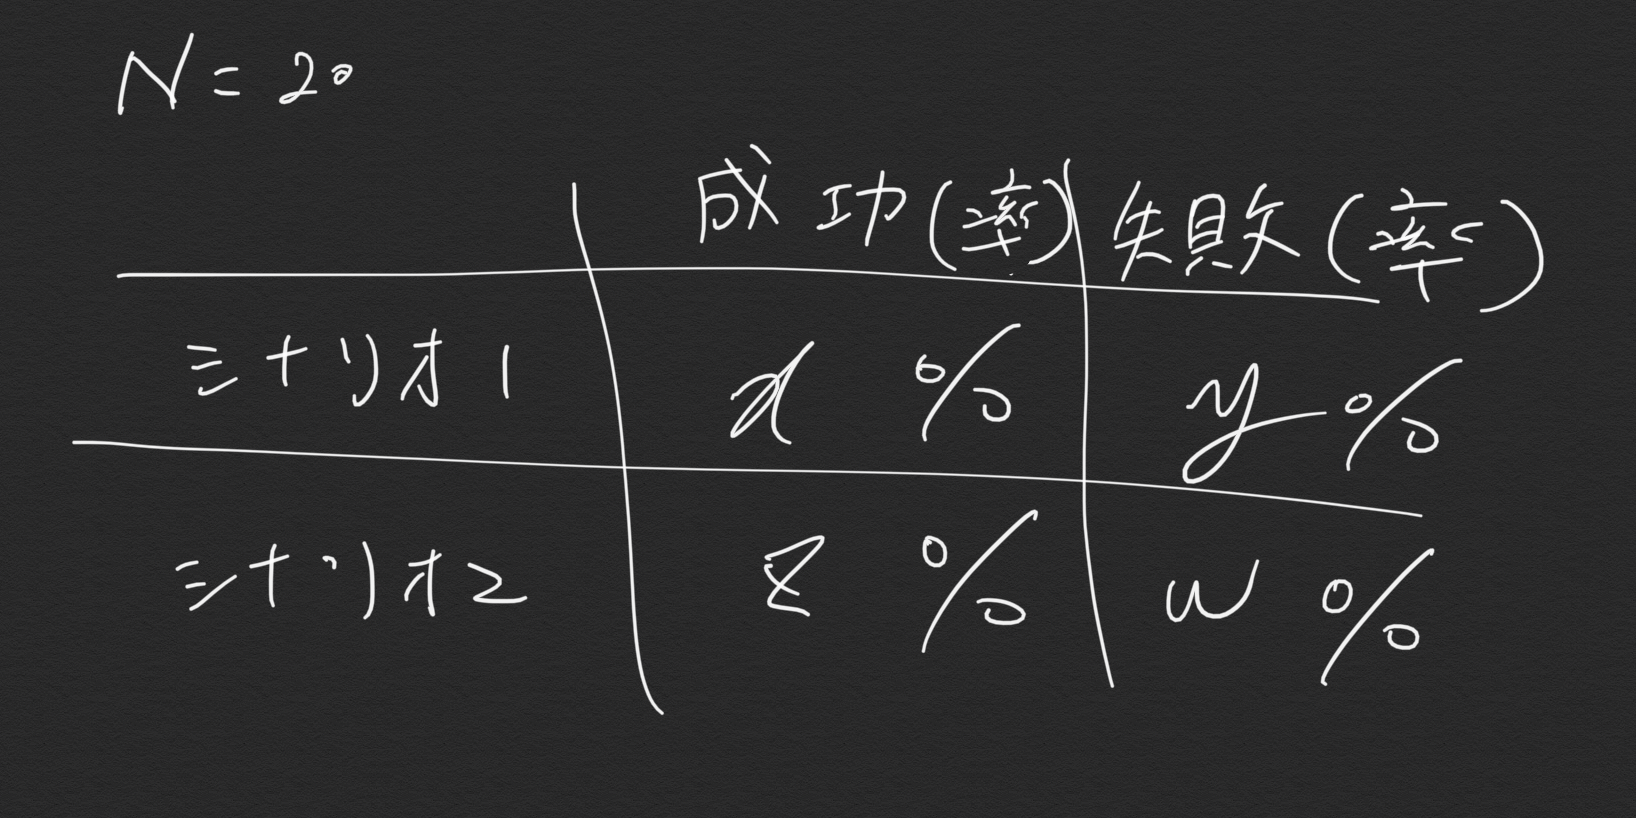
\includegraphics[bb=0 0 1000 450,width=20cm]{assets/notify_success_failure_rate.png}
  \end{center}
\end{figure}

\subsection{考察}

上記に出した結果をもとに、考察を述べる。

